
\large{Glossar UML Case Diagramm}

\begin{center}
    \begin{tikzpicture}
        \begin{umlsystem}[x=4, fill=red!10]{\systemname}
            \umlusecase[y=-10, x= 7, name=overviewcards]{Overview Cards}
            \umlusecase[y=-8.5, x=10, name=sorting]{Alphabetical sorting}
            \umlusecase[y=-14, x=9, name=filtering]{Filter function}
            \umlusecase[y=-14.5, x=1.5,  name=dSorting]{Sorting function}
            \umlusecase[y=-15.5, x=5,  name=hide]{(Un)hide function}
            \umlusecase[y=-13.5, x=0,  name=display]{Display columns}
            \umlusecase[y=-11.5, x=-1,  name=colType]{Type}
            \umlusecase[y=-12, x=1,  name=colCreatedAt]{CreatedAt}
            \umlusecase[y=-11, x=2.5,  name=colQuestion]{Question}
            \umlusecase[y=-12.5, x=-1,  name=colAnswer]{Answer}
            \umlusecase[y=-10.5, x=0.5,  name=colCntDecks]{Count of Decks}
            \umlusecase[y=-15,x=10,  name=filterCategories]{Categories}
            \umlusecase[y=-12.5,x=10, name=filterWords]{Tags}
            \umlusecase[y=-13,x=8,  name=filterSearchWords]{Search words}
            \umlusecase[y=-19, x=-1,  name=showCard]{Show card}
            \umlusecase[y=-21, x=8,  name=selectCard]{Do (Multi)select}
            
              \umlusecase[y=-22, x=8,  name=cardActions1]{Edit/Delete Card(s)}
            \umlusecase[y=-19.5, x=7,  name=cardActions2]{Create Card}
             \end{umlsystem}

        % Actors
        \umlactor[y=-6]{User}
        \umlactor[x=17.5, y=-6]{\servername}

        % Card Related
    \umlassoc[geometry=|-]{\clientname}{overviewcards}
    \umlassoc[geometry=|-]{\servername}{overviewcards}
    \umlextend{filtering}{overviewcards}
    \umlinclude{overviewcards}{sorting}
    \umlinclude{overviewcards}{display}
    \umlinherit{colType}{display}
    \umlinherit{colAnswer}{display}
    \umlinherit{colCntDecks}{display}
    \umlinherit{colQuestion}{display}
    \umlinherit{colCreatedAt}{display}
    \umlextend{selectCard}{overviewcards}
    \umlextend{hide}{overviewcards}
    \umlinherit{filterCategories}{filtering}
    \umlinherit{filterWords}{filtering}
    \umlinherit{filterSearchWords}{filtering}
    \umlassoc{cardActions1}{selectCard}
    \umlextend{showCard}{overviewcards}
    \umlextend{dSorting}{overviewcards}
    \umlextend{cardActions2}{overviewcards}
    \umlassoc[geometry=|-]{\clientname}{cardActions1}
    \umlassoc[geometry=|-]{\clientname}{cardActions2}
    \umlassoc[geometry=|-]{\clientname}{showCard}
   
    \end{tikzpicture}
\end{center}
      

\begin{answer}
    Detailanwendungsfall Einzelkartenansicht 
\end{answer}
\newline
\textbf{Akteure}: Lehrer Leo, (Studi Susi)
\newline
\textbf{Vorbedingungen}: 
\begin{itemize}  
    \item Das System ist gestartet.
    \item Leo ist angemeldet und möchte seine bereits erstellten Karteikarten einsehen. 
    Er glaubt, dass er sich bei der Karteikarte \dq Bundesländer Deutschland\dq bei der Antwort vertippt hat und möchte diese nachträglich einsehen und ggfs. anpassen, bevor er dazu einen Karteikasten für seinen Schüler Sam erstellt.
\end{itemize} 
\vspace{0,2cm}
\textbf{Nachbedingungen}: 
\begin{itemize}  
    \item Die Karte ist in der Detailansicht geöffnet.
    \item Oder: Karte ist nicht vorhanden
\end{itemize}
\vspace{0,5cm}
\textbf{Regulärer Ablauf}: 
\begin{enumerate}  
    \item Leo öffnet sein Karteikartenglossar.

        \begin{center}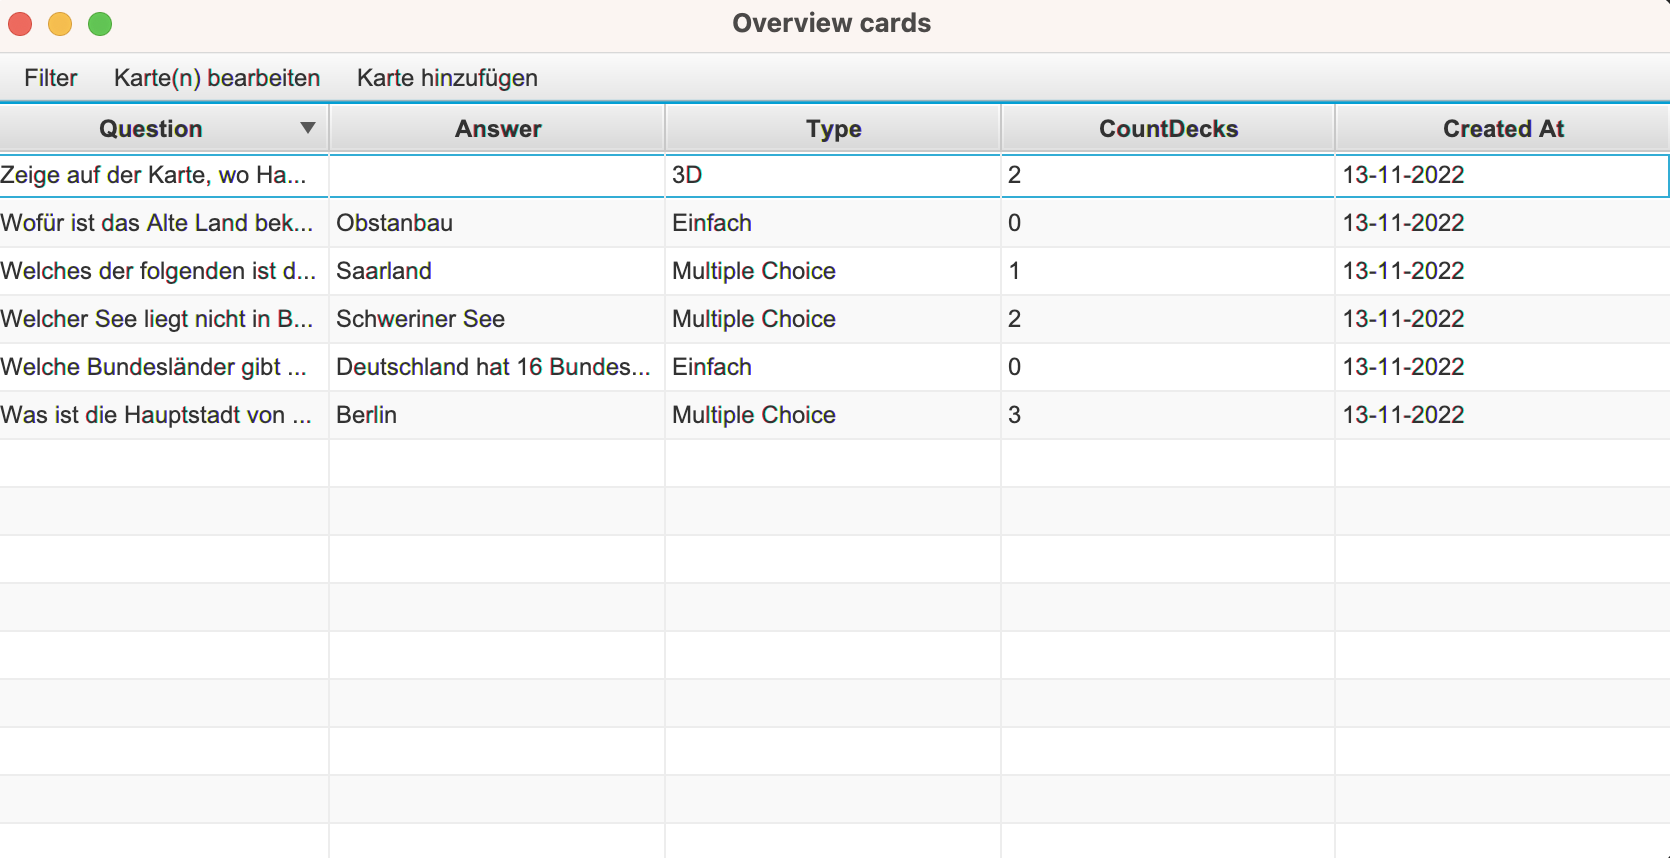
\includegraphics[width=17cm,height=35cm,keepaspectratio]{images/overview-details1.png}\end{center} 
       
    \item Er scrollt durch sein Glossar und sucht nach der Karte.
    \item Er entdeckt die gewünschte Karte und markiert sie.
    \item Er klickt auf den Button \dq Einzelkartenansicht\dq.
    \begin{center}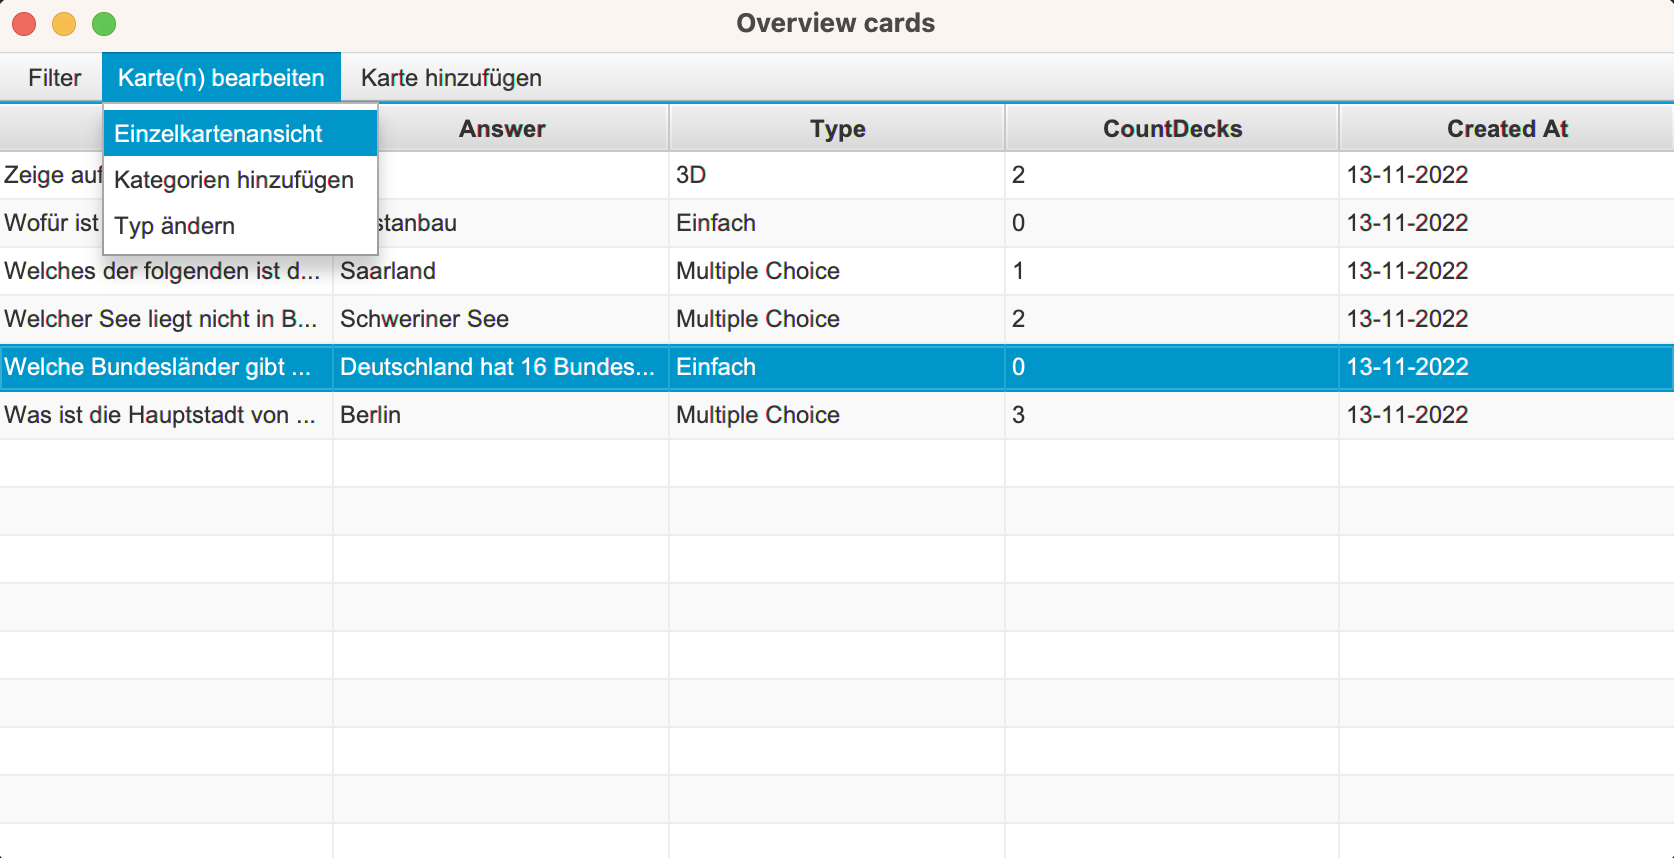
\includegraphics[width=17cm,height=35cm,keepaspectratio]{images/overview-details2.png}\end{center} 
    
    \item Er kann die Karte samt Details in einem neuen Fenster einsehen und bekommt dort alle Bearbeitungsoptionen der Karten zur Auswahl.
    \begin{center}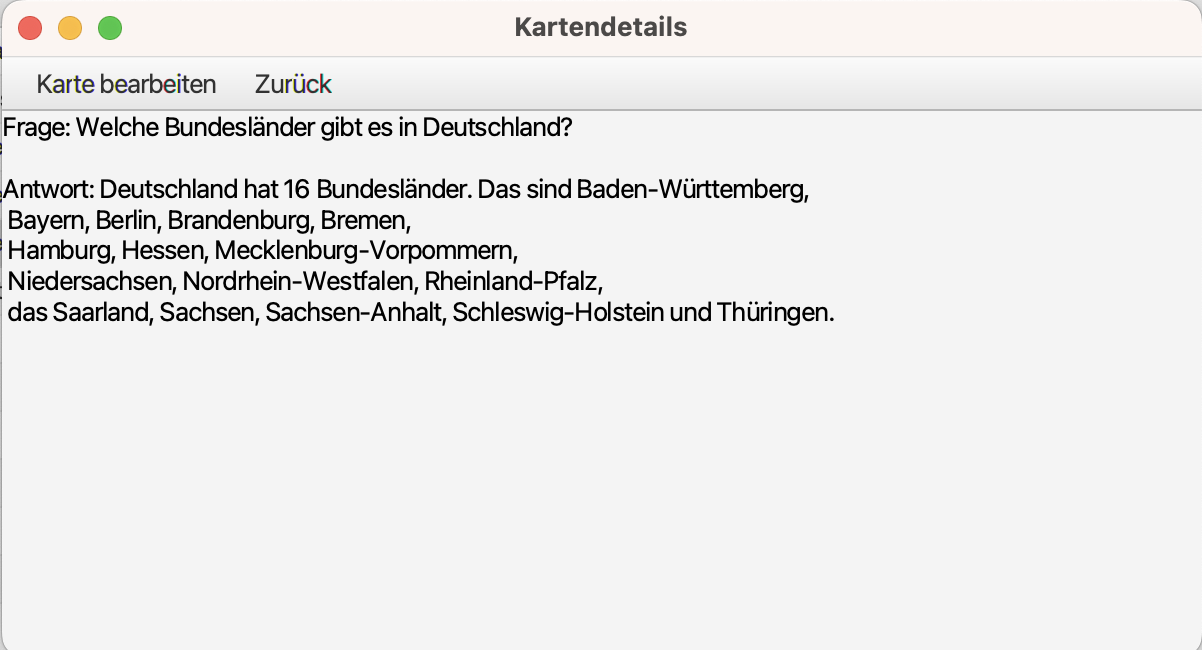
\includegraphics[width=17cm,height=35cm,keepaspectratio]{images/overview-details3.png}\end{center} 
       
\end{enumerate} 
\textbf{Alternative}:
\newline Zu 3. Da er die Karte auf Anhieb nicht findet, filtert er durch die Suchwörter mittels Eingabe von \dq Bundesländer Deutschland\dq nach der gewünschten Karte.
\newline Zu 3. Die gewünschte Karte existiert nicht. Leo legt stattdessen eine neue über den Button \dq Karte anlegen\dq an.
